\documentclass[journal,12pt,twocolumn]{IEEEtran}
\IEEEoverridecommandlockouts
\usepackage{setspace}
\usepackage{gensymb}
\singlespacing
\usepackage[cmex10]{amsmath}
\usepackage{amsthm}
\usepackage{mathrsfs}
\usepackage{txfonts}
\usepackage{stfloats}
\usepackage{bm}
\usepackage{cite}
\usepackage{cases}
\usepackage{subfig}
\usepackage{longtable}
\usepackage{multirow}
\usepackage{enumitem}
\usepackage{mathtools}
\usepackage{tikz}
\usepackage{circuitikz}
\usepackage{verbatim}
\usepackage[breaklinks=true]{hyperref}
\usepackage{tkz-euclide} % loads  TikZ and tkz-base
\usepackage{listings}
\usepackage{color}    
\usepackage{array}    
\usepackage{longtable}
\usepackage{calc}     
\usepackage{multirow} 
\usepackage{hhline}   
\usepackage{ifthen}   
\usepackage{lscape}     
\usepackage{chngcntr}
\usepackage{algorithm}
\usepackage[indLines=false]{algpseudocodex}
\DeclareMathOperator*{\Res}{Res}
\renewcommand\thesection{\arabic{section}}
\renewcommand\thesubsection{\thesection.\arabic{subsection}}
\renewcommand\thesubsubsection{\thesubsection.\arabic{subsubsection}}

\renewcommand\thesectiondis{\arabic{section}}
\renewcommand\thesubsectiondis{\thesectiondis.\arabic{subsection}}
\renewcommand\thesubsubsectiondis{\thesubsectiondis.\arabic{subsubsection}}
\renewcommand\thetable{\arabic{table}}
% correct bad hyphenation here
\hyphenation{op-tical net-works semi-conduc-tor}
\def\inputGnumericTable{}                                 %%

\renewcommand\algorithmicensure{\textbf{Input:}}
\newcommand{\algorithmautorefname}{Algorithm}

\lstset{
%language=C,
frame=single, 
breaklines=true,
columns=fullflexible,
literate=
{-}{$\rightarrow{}$}{1},
}
%\lstset{
%language=tex,
%frame=single, 
%breaklines=true
%}

\DeclareMathOperator*{\argmax}{arg\,max}
\DeclareMathOperator*{\argmin}{arg\,min}
\begin{document}
\newtheorem{theorem}{Theorem}[section]
\newtheorem{problem}{Problem}
\newtheorem{proposition}{Proposition}[section]
\newtheorem{lemma}{Lemma}[section]
\newtheorem{corollary}[theorem]{Corollary}
\newtheorem{example}{Example}[section]
\newtheorem{definition}[problem]{Definition}
\newcommand{\BEQA}{\begin{eqnarray}}
\newcommand{\EEQA}{\end{eqnarray}}
\newcommand{\define}{\stackrel{\triangle}{=}}
\bibliographystyle{IEEEtran}
\providecommand{\mbf}{\mathbf}
\providecommand{\pr}[1]{\ensuremath{\Pr\left(#1\right)}}
\providecommand{\qfunc}[1]{\ensuremath{Q\left(#1\right)}}
\providecommand{\sbrak}[1]{\ensuremath{{}\left[#1\right]}}
\providecommand{\lsbrak}[1]{\ensuremath{{}\left[#1\right.}}
\providecommand{\rsbrak}[1]{\ensuremath{{}\left.#1\right]}}
\providecommand{\brak}[1]{\ensuremath{\left(#1\right)}}
\providecommand{\lbrak}[1]{\ensuremath{\left(#1\right.}}
\providecommand{\rbrak}[1]{\ensuremath{\left.#1\right)}}
\providecommand{\cbrak}[1]{\ensuremath{\left\{#1\right\}}}
\providecommand{\lcbrak}[1]{\ensuremath{\left\{#1\right.}}
\providecommand{\rcbrak}[1]{\ensuremath{\left.#1\right\}}}
\theoremstyle{remark}
\newtheorem{rem}{Remark}
\newcommand{\sgn}{\mathop{\mathrm{sgn}}}
\providecommand{\abs}[1]{\left\vert#1\right\vert}
\providecommand{\res}[1]{\Res\displaylimits_{#1}} 
\providecommand{\norm}[1]{\left\lVert#1\right\rVert}
\providecommand{\mtx}[1]{\mathbf{#1}}
\providecommand{\mean}[1]{E\left[ #1 \right]}   
\providecommand{\fourier}{\overset{\mathcal{F}}{ \rightleftharpoons}}
\providecommand{\system}[1]{\overset{\mathcal{#1}}{ \longleftrightarrow}}
\newcommand{\solution}{\noindent \textbf{Solution: }}
\newcommand{\cosec}{\,\text{cosec}\,}
\providecommand{\dec}[2]{\ensuremath{\overset{#1}{\underset{#2}{\gtrless}}}}
\newcommand{\myvec}[1]{\ensuremath{\begin{pmatrix}#1\end{pmatrix}}}
\newcommand{\mydet}[1]{\ensuremath{\begin{vmatrix}#1\end{vmatrix}}}
\renewcommand{\vec}[1]{\boldsymbol{\mathbf{#1}}}
\def\putbox#1#2#3{\makebox[0in][l]{\makebox[#1][l]{}\raisebox{\baselineskip}[0in][0in]{\raisebox{#2}[0in][0in]{#3}}}}
     \def\rightbox#1{\makebox[0in][r]{#1}}
     \def\centbox#1{\makebox[0in]{#1}}
     \def\topbox#1{\raisebox{-\baselineskip}[0in][0in]{#1}}
     \def\midbox#1{\raisebox{-0.5\baselineskip}[0in][0in]{#1}}

\vspace{3cm}
\title{Beacon Tracking Using ESP32}
\author{
    \IEEEauthorblockN{Gautam Singh, G.V.V. Sharma} \\
    \IEEEauthorblockA{Indian Institute of Technology Hyderabad, India} \\
    Email: cs21btech11018@iith.ac.in, gadepall@ee.iith.ac.in
}
\maketitle
% \tableofcontents
\bigskip

\begin{abstract}
    This document is a report which demonstrates the use of machine learning
    in beacon tracking using an unmanned ground vehicle (UGV) and a WiFi-enabled
    microcontroller such as the ESP32.
\end{abstract}

\section{Assets}
\begin{enumerate}
    \item UGV chassis with DC motors
    \item ESP32 microcontroller with Type-B USB cable
    \item L293D Motor Driver IC
    \item Breadboard and Jumper Wires
    \item Android phone
    \item (Optional) USB 2.0/3.0 Hub
\end{enumerate}

\section{Procedure}
\begin{enumerate}
    \item Make the connections as per the wiring diagram in Fig. \ref{fig:beacon}.
    \item Connect the ESP32 board to your Android Phone.
    \item Generate the firmware by entering the following commands.
        \begin{lstlisting}
$ cd codes
$ pio run
        \end{lstlisting}
    \item Go to ArduinoDroid and select
        \begin{lstlisting}
Actions - Upload - Upload Precompiled
        \end{lstlisting}
    and choose the firmware file at
        \begin{lstlisting}
codes/.pio/build/firmware.hex
        \end{lstlisting}
    \item Now put the phone at a reasonable distance from the UGV with no 
    obstacles in the way and then turn on the hotspot. The UGV should travel
    towards the phone and stop near it.
\end{enumerate}

\begin{figure}[!ht]
    \centering
    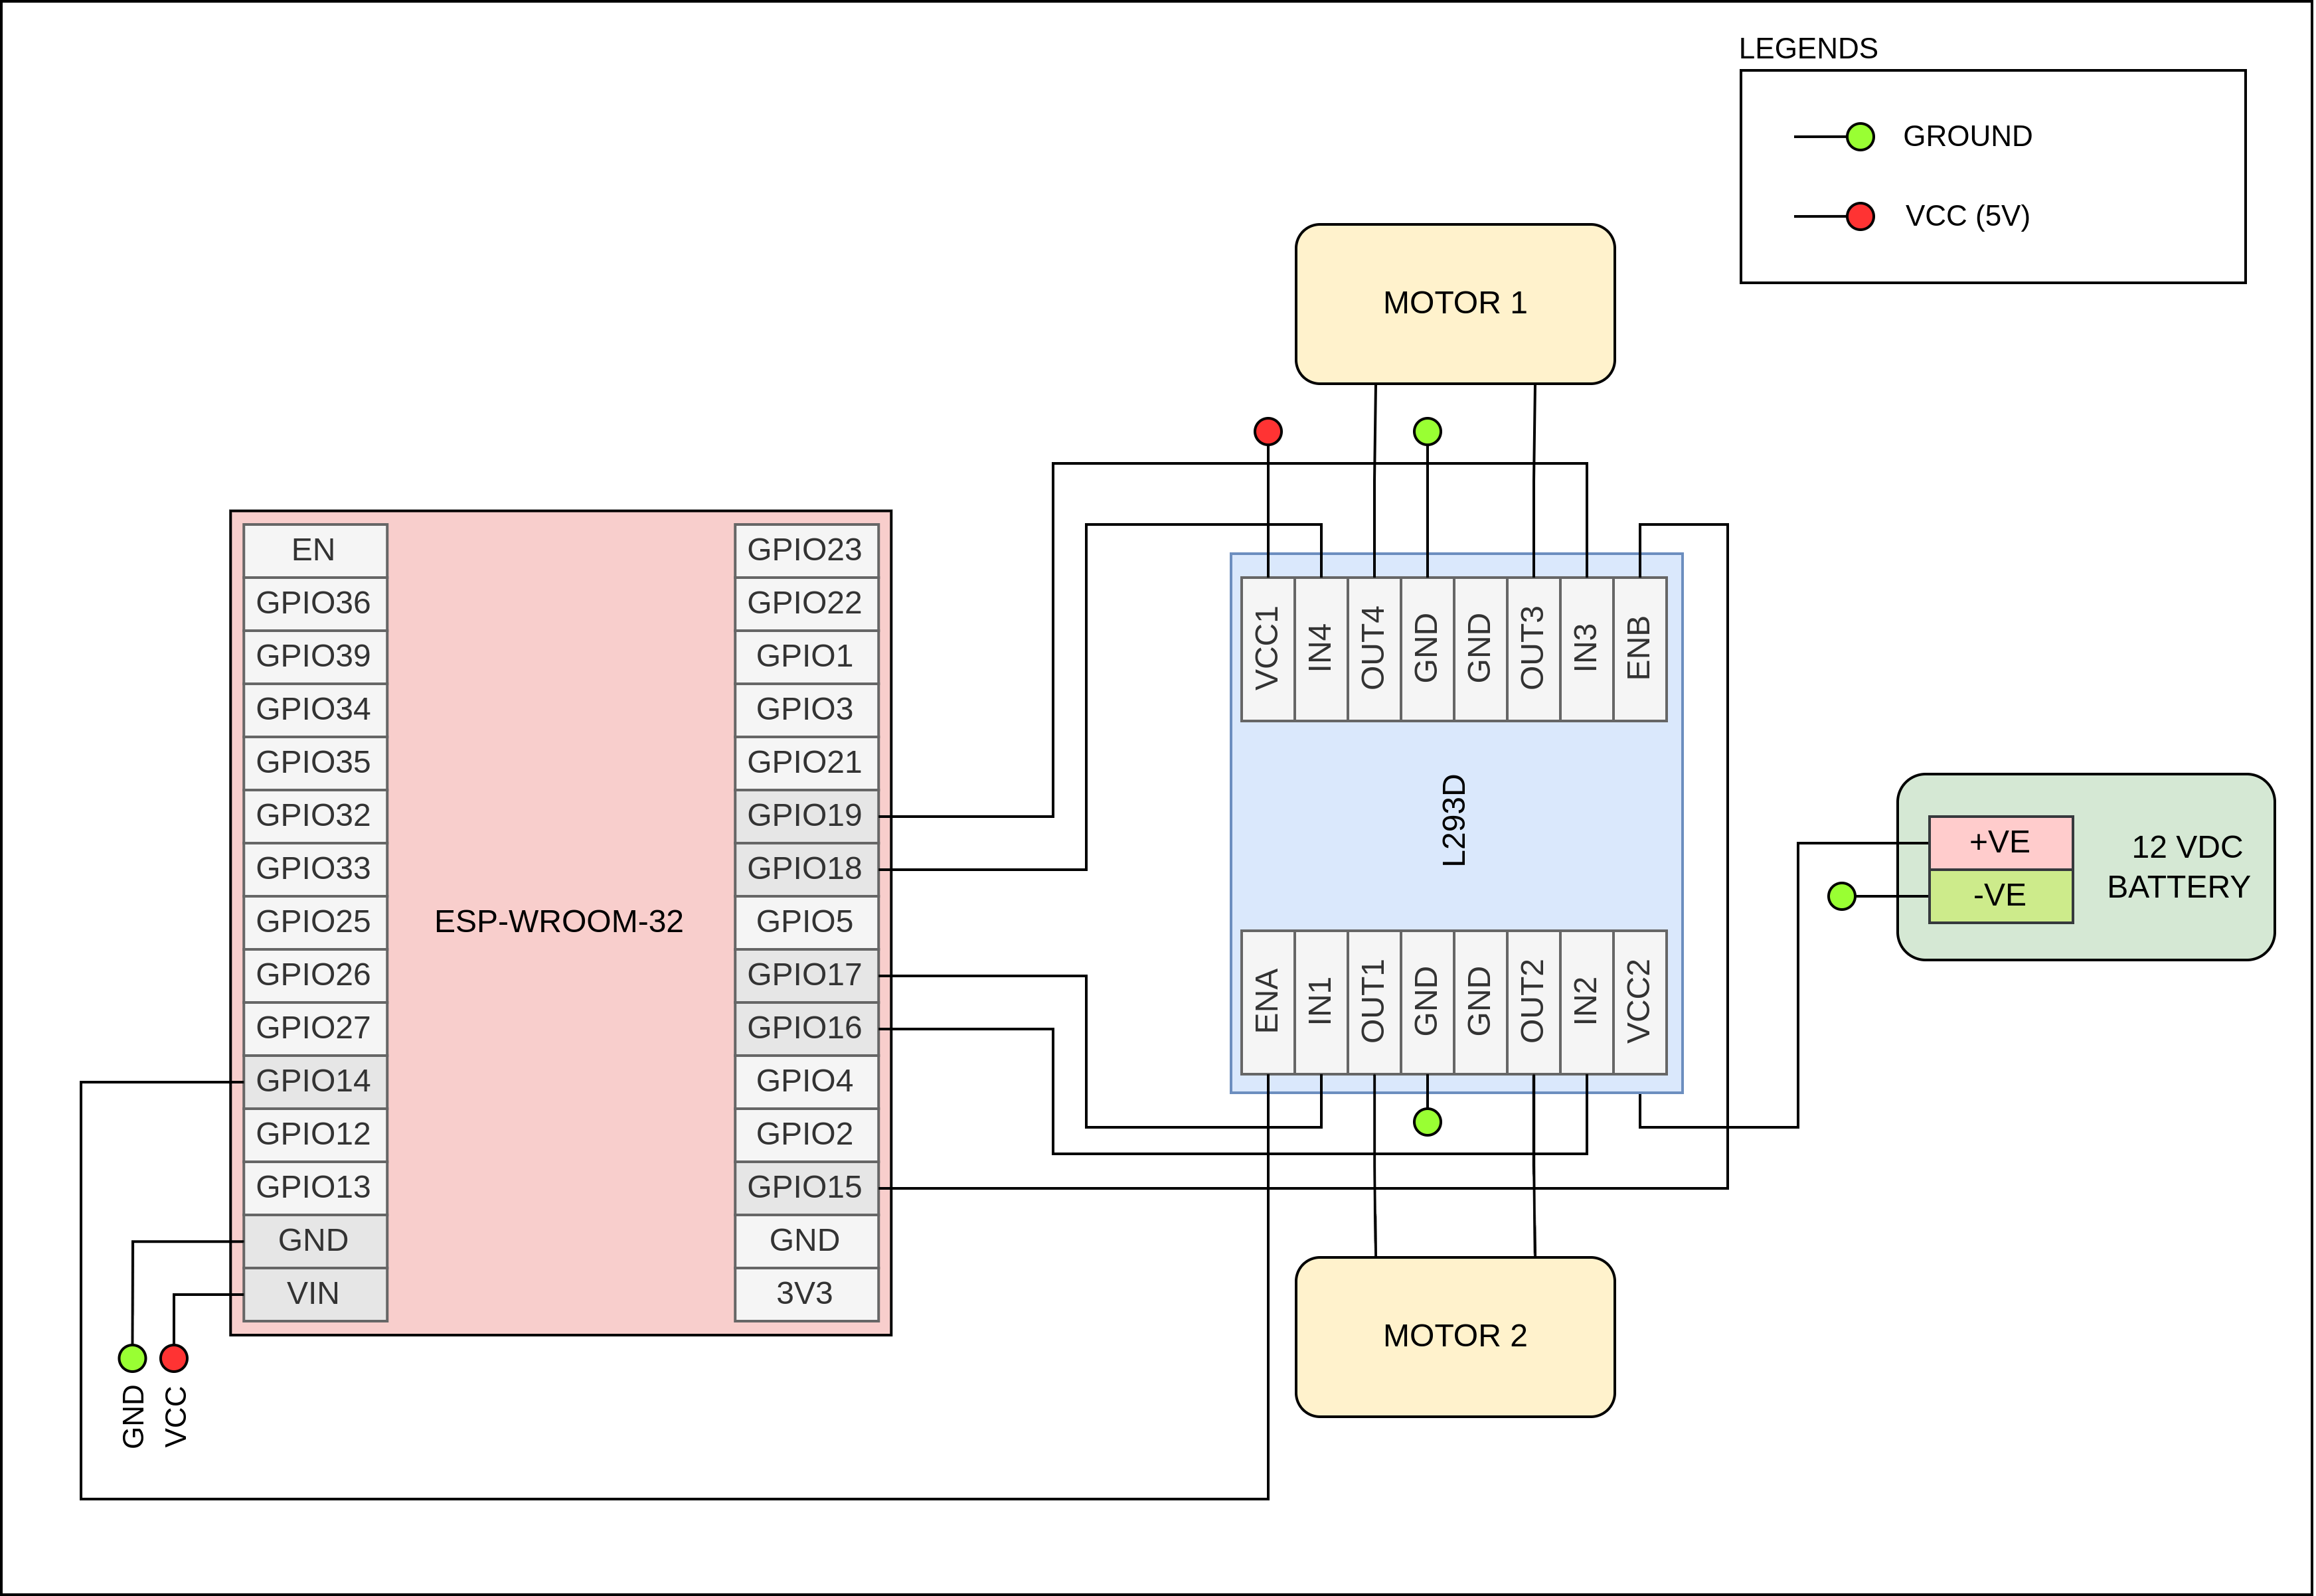
\includegraphics[width=\columnwidth]{figs/beacon.png}
    \caption{Wiring Diagram for Beacon Tracking.}
    \label{fig:beacon}
\end{figure}

\section{Working}
To estimate (radial) distance to beacon, we use its signal strength. For WiFi,
this is the \textbf{Received Signal Strength Indicator} (RSSI). The RSSI (in
dBm) at radial distance of \(r\) metres is given by
\begin{align}
    R\brak{r} = R\brak{1} - 10\log_{10}\brak{r}
    \label{eq:rssi}
\end{align}
where \(R(1)\) is the RSSI at a distance of 1 metre from the beacon. Clearly,
\(R\brak{r}\) is a decreasing function as \(\log_{10}\brak{r}\) is an increasing
function. Further, the second derivative of \(R\brak{r}\) is given by
\begin{equation}
    \frac{d^2R\brak{r}}{dr^2} = \frac{10}{\ln{10}}\frac{1}{r^2} > 0.
    \label{eq:rssidd}
\end{equation}
Clearly, the RSSI is a convex function of the radial distance \(r\). This
implies that we can use gradient ascent to find the point where the RSSI is
maximum, which would be the location of the beacon. The UGV uses a recursive
algorithm to update its position using this principle until it is close enough
to the beacon based on the RSSI measurements it takes at various points in its
vicinity. The algorithm is described in \autoref{alg:beacon}.

\begin{algorithm}[H]
    \caption{Beacon Tracking Algorithm}
    \label{alg:beacon}
    \begin{algorithmic}[1]
        \Ensure{RSSI threshold \(T\), number of steps \(N\)}
        \While{\textsc{GetRSSI()} \(< T\)}
            \State Take \(N\) steps in a straight line and measure the RSSI at 
            each step.
            \State Suppose the maximum RSSI is measured at step \(i\).
            \State Move to the position at step \(i\)
            \If{\(i = N\)}
                \State Move one step forward.
            \ElsIf{\(i = 0\)}
                \State Move one step backward.
            \Else
                \State Turn left.
            \EndIf
        \EndWhile
    \end{algorithmic}
\end{algorithm}

\section{Observations}
The UGV eventually converges close to the beacon (here, the hotspot). However,
if there are a lot of nearby obstacles, the UGV may not converge close to the
location of the beacon. It may either get physically blocked by the beacon or
the signal interference may be too high.

\end{document}
